\documentclass{article}
\usepackage[utf8]{inputenc}
\usepackage[margin=1in]{geometry} 
\usepackage{graphicx}
\usepackage{caption}
\usepackage{subcaption}
\title{Experiments on new Data}
\author{Florian Kneifel}
\date{July 2021}

\begin{document}



\section{Experiments on non-image data}
For this badge please refer to the notebook "captum\textunderscore on\textunderscore timeseries.ipynb" 

\subsection{data}
As a simple toy-dataset for timeseries data, we use the "flights" dataset that comes with the seaborn library. The dataset contains the number of flight passengers per month for the years 1949 to 1960. So in total there are 144 datapoints. Just by looking at the data we can see a yearly pattern, but also a steady increase on a macro scale. Also for easier use the data in the notebook gets normalized before training a model. The task will be set up as a regression problem: The model gets the data from the last 10 months and has to predict the next month. Note that here we intentionally used a window smaller than 12, because otherwise the task will become to easy because of the intra-year-pattern.

\subsection{simple linear model}
For the first experiment we use a realatively simple linear model with the following architecture: 
\begin{itemize}
\item Input of size 10
\item Linear-Layer with 3 neurons
\item Sigmoid-Layer
\item Linear-Layer with 1 neuron
\end{itemize}

Considering the simplicity of the model, we get pretty accurate predictions:

\begin{figure}[h!]
\centering
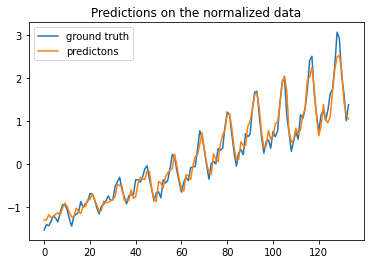
\includegraphics[scale=0.6]{linear_model_prediction}
\caption{linear model performance}
\label{fig:lin_model_perf}
\end{figure}

First we can look at which input feature on average has the most importance for the prediction:

\begin{figure}[ht!]
\centering
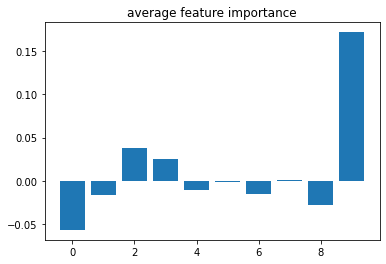
\includegraphics[scale=0.6]{linear_model_avg_feature_importance.png}
\caption{average feature importance}
\label{fig:lin_model_afi}
\end{figure}

There seems to be a pretty strong focus from the network towards the input at index 9. That is not surprising, considering that the number of flights most of the time is not drastically different from the last month. Looking at the average importance of neuron 0 in \ref{fig:lin_model_ani} and the negative corellation of almost every input for neuron 0 in \ref{fig:lin_model_anfi} one might conclude, that neuron 0 is trained to predict a decline, while neuron 1 and especially neuron 2 are mostly predicting increasing flight passengers.

\begin{figure}[h!]
     \centering
     \begin{subfigure}[b]{0.2\textwidth}
         \centering
         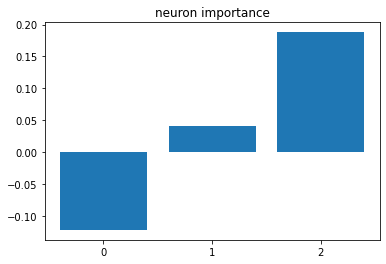
\includegraphics[scale=0.4]{linear_model_avg_neuron_importance.png}
         \caption{neuron importance}
         \label{fig:lin_model_ani}
     \end{subfigure}
     \hspace*{\fill}
     \begin{subfigure}[b]{0.4\textwidth}
         \centering
         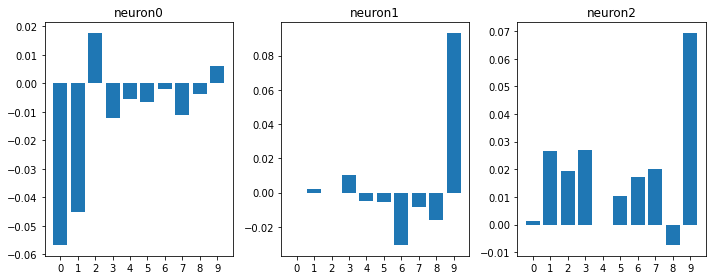
\includegraphics[scale=0.4]{linear_model_avg_feature_per_neuron_importance.png}
         \caption{average feature importance per neuron}
         \label{fig:lin_model_anfi}
     \end{subfigure}
     \hspace*{\fill}
        \caption{average importance}
        \label{fig:lin_model_a_f_i}
\end{figure}


\subsubsection{Pattern recognition}

Because of the way the data is organized, we can use a step size of 12 to get the same month for consecutive years. At first sight, we might assume that there is a certain regularity in the way the inputs are interpreted. But if we use a random model to repeat the same experiment, we see a similar patterns emerging. (however because the attributions are way smaller a factor 10 is added to the visualization) In conclusion, we can not really get any insight in the pattern recognition performed by the neural network from this experiment.



For the last experiment we use a CNN to better resemble an architecture, that one would also find for image tasks. Just comparing the different methods provided by Captum shows quite different results. Especially looking at the input at index 9 shows a strong positive signal from the method "saliency" but is negative for "integrated gradients" and "deep lift".


All in all it is interesting to see which neuron behaves which way, and how the input features are correlated to the output. However interpreting the workings of the neural net from this information is not possible. For this timeseries-task it is even harder, because even with a lot of training we as humans can not simply look at a short timeseries plot and predict the next value. At picture classification humans are naturally gifted and can generally perform well.




\end{document}
